\documentclass{beamer}

% Theme
\usetheme{Madrid}
\usepackage{fontawesome5}
\usecolortheme{default}
\usepackage{tikz}
\usepackage{amsmath}
\usetikzlibrary{shapes.geometric, backgrounds}
\usetikzlibrary{arrows.meta, positioning} % For arrows and 
\usepackage{amssymb}

\usetikzlibrary{positioning} % For node positioning
\usetikzlibrary{calc} % For calculations in TikZ
\usetikzlibrary{math} 


\usetikzlibrary{decorations.pathreplacing, arrows.meta}
% For colored boxes
\usepackage{xcolor}%positioning


\definecolor{hotpink}{RGB}{255, 105, 180}
\definecolor{neonyellow}{RGB}{255, 255, 0}
\definecolor{brightorange}{RGB}{255, 165, 0}
\definecolor{brightpurple}{RGB}{128, 0, 128}
\definecolor{turquoise}{RGB}{64, 224, 208}

% Packages
\usepackage{graphicx}

% Remove the default footer
\setbeamertemplate{footline}[frame number]
\setbeamercolor{block title}{bg=blue!50, fg=white} % Title background blue with white text
\setbeamercolor{block body}{bg=blue!10, fg=black} % Body background light blue with black text


\setbeamertemplate{footline}{%
    \leavevmode%
    \hbox{%
        % Left side: Name
        \begin{beamercolorbox}[wd=0.33\paperwidth,ht=2.5ex,dp=1.5ex,leftskip=1em]{author in head/foot}%
            \usebeamerfont{author in head/foot}%
            Niloy, Shovon
        \end{beamercolorbox}%
        % Center: BUET
        \begin{beamercolorbox}[wd=0.34\paperwidth,ht=2.5ex,dp=1.5ex,center]{title in head/foot}%
            \usebeamerfont{title in head/foot}%
            BUET
        \end{beamercolorbox}%
        % Right side: Page number
        \begin{beamercolorbox}[wd=0.33\paperwidth,ht=2.5ex,dp=1.5ex,rightskip=1em]{title in head/foot}%
            \usebeamerfont{title in head/foot}%
            \insertframenumber{} / \inserttotalframenumber%
        \end{beamercolorbox}%
    }%
}



% Title details
\title{Data Encryption Standard}
\subtitle{The Chamber of Secrets: Guarding Digital Realms}
\author{Niloy Kumar Mondal, Monjur Hossain Khan Shovon}
\institute[BUET]{Bangladesh University of Engineering \& Technology}
\date{November 24, 2024}

\begin{document}

% Title slide
 \begin{frame}
    \titlepage
    \begin{center}
        % Optionally, include a logo
         % \includegraphics[width=2cm]{cse_buet.png}
    \end{center}
 \end{frame}

% Content Slide with Hyperlinks (Table of Contents)
\begin{frame}
    \frametitle{Table of Contents}
    \tableofcontents
\end{frame}

% Section 1 - Overview
\section{Overview}

% Slide 1: Blurred Purpose Block
\begin{frame}
    \frametitle{Overview: What is Encryption?}
    \label{sec:what_is_encryption}

    \begin{block}{Definition}
        Encryption is the process of converting readable data into an unreadable format, ensuring that only authorized parties can access the information.
    \end{block}

    % The blurred purpose block (overlay technique using TikZ)
    \begin{tikzpicture}[overlay, remember picture]
        \node[fill=gray, opacity=0.3, text width=0.8\textwidth, align = bottom, anchor=center] at (current page.center) {
            \begin{minipage}{\textwidth}
                \textbf{Purpose} \\
                It ensures confidentiality, integrity, and security of data during storage or transmission.
            \end{minipage}
        };
    \end{tikzpicture}
\end{frame}

% Slide 2: Unblurred Purpose Block
\begin{frame}
    \frametitle{Overview: What is Encryption?}
    \label{sec:what_is_encryption_revealed}

    \begin{block}{Definition}
        Encryption is the process of converting readable data into an unreadable format, ensuring that only authorized parties can access the information.
    \end{block}

    \begin{block}{Purpose}
        It ensures confidentiality, integrity, and security of data during storage or transmission.
    \end{block}
\end{frame}




\begin{frame}
    \frametitle{Overview: Why Do We Need Encryption?}
    \label{sec:why_encryption}

    \begin{exampleblock}{Reasons for Encryption}
        \begin{itemize}
            \item Safeguards sensitive information like personal data and financial transactions.
            \item Prevents unauthorized access and protects against data breaches.
            \item Maintains privacy and confidentiality in an increasingly digital world.
        \end{itemize}
    \end{exampleblock}
\end{frame}


\begin{frame}
    \frametitle{Overview: Risks Without Encryption}
    \label{sec:risks_without_encryption}

    \begin{alertblock}{What Happens Without Encryption?}
        \begin{itemize}
            \item Sensitive data can be intercepted during transmission.
            \item Leads to privacy violations, identity theft, and financial loss.
            \item Vulnerable systems are easy targets for hackers and attackers.
        \end{itemize}
    \end{alertblock}
\end{frame}





% Section 2 - What is Data Encryption?
\section{What is Data Encryption Standard(DES)?}
\begin{frame}
    \frametitle{What is Data Encryption Standard(DES)?}
    \label{sec:data_encryption}
    % Content for this section
    Data encryption transforms readable data into an unreadable format to protect confidentiality.
\end{frame}

% Section 3 - Why do we need this?
\section{Why do we need this?}
\begin{frame}
    \frametitle{Why do we need this?}
    \label{sec:need}
    % Content for this section
    Here, we explore why encryption is vital in securing digital data.
\end{frame}

% Section 4 - Algorithm
\section{Algorithm}
\begin{frame}
    \frametitle{Algorithm}
    \label{sec:algorithm}
    % Content for this section
    Discussing the working of the DES algorithm.
\end{frame}

% Section 5 - Pseudocode
\section{Algorithm}
\begin{frame}
    \frametitle{Algorithm}
    \label{sec:pseudocode}
     \setbeamercovered{transparent}
    \begin{block}{Pseudocode : Data Encryption Standard (DES)}
    \begin{enumerate}
        \item<1-> \textbf{Input:} 64-bit plaintext block $P$, 56-bit main key $K$.
        \item<2-> Generate 16 round sub-keys $K_1, K_2, \ldots, K_{16}$ from $K$.
        \item<3-> Apply initial permutation (IP) on $P$ to get $L_0$ and $R_0$.
        \item<4-> \textbf{for} $i \gets 1$ to $16$ \textbf{do}  
        \begin{itemize}
            \item<5-> Compute $L_i \gets R_{i-1}$.
            \item<6-> Compute $R_i \gets L_{i-1} \oplus f(R_{i-1}, K_i)$.
        \end{itemize}
        \item<7-> \textbf{end for}
        \item<8-> Combine $R_{16}$ and $L_{16}$.
        \item<9-> Apply inverse initial permutation (IP$^{-1}$).
        \item<10-> \textbf{Output:} 64-bit ciphertext block $C$.
    \end{enumerate}
    \end{block}
\end{frame}


\section{Algorithm Visualization}
\begin{frame}
    \frametitle{(DES) Algorithm Simulation}
    \label{sec:algorithm_flow}
        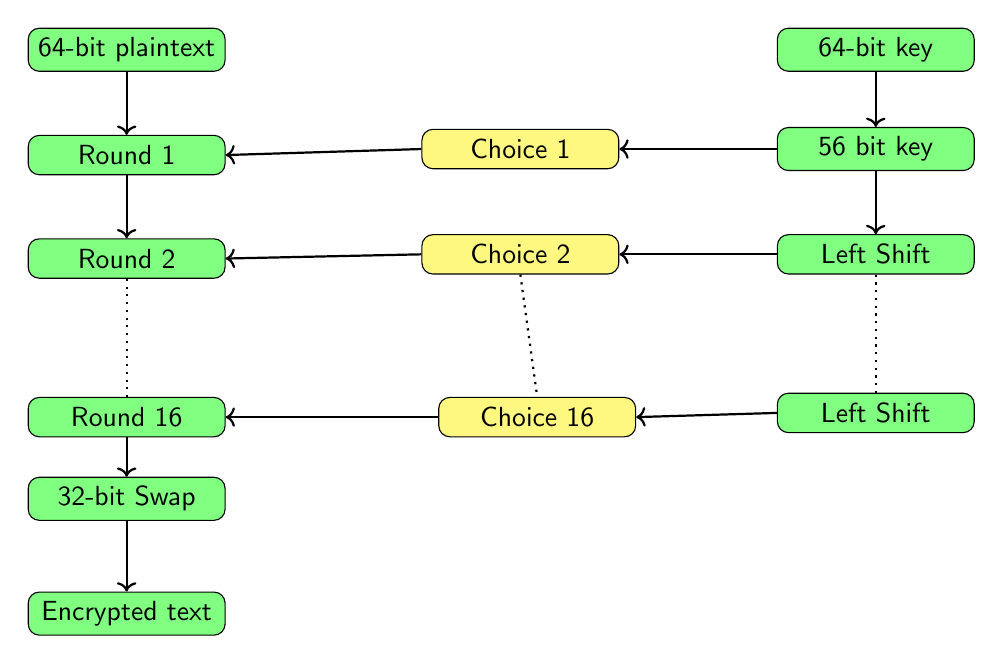
\begin{tikzpicture}[
    every node/.style={align=center},
    arrow/.style={-Triangle, thick},
    brace/.style={decorate, decoration={brace, amplitude=5pt}},
    custom/.style={
                draw, 
                rounded corners,  
                minimum width=2.5cm, 
                minimum height=0.5cm, 
                font=\sffamily,
                fill=green!50
            },
     custom2/.style={
                draw, 
                rounded corners,  
                minimum width=2.5cm, 
                minimum height=0.5cm, 
                font=\sffamily,
                fill=yellow!50
            }
    ]

    \visible<1->
    {
    
\node[custom] (plaintext) {64-bit plaintext};
\node[custom, right=7cm of plaintext] (Ikey) {64-bit key}; 
    
    }

    \visible<2->
    {
      \node[custom,below = 6.6cm of plaintext] (ent) {Encrypted text};
    }

    \visible<3->
    {
          \node[custom,below=0.7cm of Ikey](K1) {56 bit key};
          \draw[->, thick] (Ikey.south) -- (K1.north);
    }
    \visible<4->
    {
         \node[custom,below=0.8cm of K1](K2){Left Shift};
         \draw[->, thick] (K1.south) -- (K2.north);
         \node[custom2,left = 2cm of K1] (c1) {Choice 1};
         \draw[->, thick] (K1.west) -- (c1.east);
    }
    \visible<5->
    {
        \node[custom,below = 0.8cm of plaintext] (r1) {Round 1};
        \draw[->, thick] (plaintext.south) -- (r1.north);
        \draw[->, thick] (c1.west) -- (r1.east);
    }
    \visible<6->
    {
          \node[custom2,left = 2cm of K2] (c2) {Choice 2};
          \draw[->, thick] (K2.west) -- (c2.east);
    }
    \visible<7->
    {
       \node[custom,below = 0.8cm of r1] (r2) {Round 2};
       \draw[->, thick] (c2.west) -- (r2.east);
       \draw[->, thick] (r1.south) -- (r2.north);
    }

    \visible<8->
    {
       \node[custom,below = 1.5cm of r2] (r16) {Round 16};
       \node[custom2,right = 2.7cm of r16] (c16) {Choice 16};\
       \node[custom,below=1.5cm of K2](K16){Left Shift};   
      \draw[dotted, thick] (K2.south) -- (K16.north);
       \draw[dotted, thick] (r2.south) -- (r16.north);
       \draw[->, thick] (c16.west) -- (r16.east);
       \draw[->, thick] (K16.west) -- (c16.east);
       \draw[dotted, thick] (c2.south) -- (c16.north);
      
    }

      \visible<9->
    {
       \node[custom,below = 0.5cm of r16] (swap) {32-bit Swap};
       \draw[->, thick] (r16.south) -- (swap.north);
       \draw[->, thick] (swap.south) -- (ent.north);
       
    }
    \end{tikzpicture}
    
    
    
\end{frame}

\begin{frame}
    \frametitle{(DES) Algorithm Single Round Visualization}
    \label{sec:algorithm_visualization}
          

    \begin{center}
        \begin{tikzpicture}[
            every node/.style={
                draw, 
                rounded corners,  
                minimum width=2.5cm, 
                minimum height=0.5cm, 
                font=\sffamily,
                fill=green!50
            },
        round/.style={
            fill=yellow!30 % Light blue background for the 'round' node
        },
        center/.style={
            fill=lightgreen!30 % Light green background for the 'Partially Encrypted Text' node
        }
        ]
            % First row node
            \node[fill=yellow!50](Round) {$round_i$};
            \visible<2->{
                        \node[fill=red!50,below =0.4cm of Round,xshift=-80] (center) {Partially Encrypted Text};
            }
            \visible<3->
            {
                           \node[below=0.7cm of center, xshift=-60] (left) {Left Half = $L_i$};
                            \node[below=0.7cm of center, xshift=60] (right) {Right Half = $R_i$};
                           \draw[->, thick] (center.south) -- (left.north);
                           \draw[->, thick] (center.south) -- (right.north);
            
            }
            \visible<4->
            {
            \node[below=3.5cm of left] (left1) {Left Half=$L_{i+1}$};
            \draw[->, thick] (right.south) -- (left1.north);
            }
            \visible<5->
            {
                             % Key node
            \node[fill=hotpink!50,below right=2.1 and 2 cm of center] (keys) {Left Shifted \faIcon{key}
 Key=K$_i$};
            }

            \visible<6->
            {
                            \node[fill=gray!60,below=0.7cm of right, draw, minimum size=0.8cm, align=center] (function) {\textit{f}};
                              \draw[->, thick] (right.south) -- (function.north);
                               \draw[->, thick] (keys.west) -- (function.east);
            }
            \visible<7->
            {
                              \node[fill=blue!50,below=0.7cm of function, draw,  shape=circle, minimum size=0.7cm, inner sep=0pt, align=center] (xor) {\Huge $\oplus$};

                              \draw[->, thick] (function.south) -- (xor.north);
                              \draw[->, thick] (left.south) -- (xor.west);  
            }

           
            \visible<8->
            {
                 \node[fill=green!50,below=3.5cm of right] (right1){Right Half=$R_{i+1}$};
                 \draw[->, thick] (xor.south) -- (right1.north);
            }


        
        \end{tikzpicture}
    \end{center}
    

\end{frame}















% Section 6 - Applications
\section{Applications}
\begin{frame}
    \frametitle{Applications}
    \label{sec:applications}
    \begin{block}{Applications of DES}
        \begin{itemize}
            \item<1-> \textbf{Secure Communication}  
            % Used in early secure messaging systems to encrypt sensitive information.
            
            \item<2-> \textbf{Banking Systems}  
            % Employed for encrypting PINs and authenticating transactions in ATMs.
            
            \item<3-> \textbf{File Encryption}  
            % Protects files during storage or transfer over insecure channels.
            
            \item<4-> \textbf{Smart Cards}  
            % Used in older smart card technologies for data protection.
            
            \item<5-> \textbf{Wireless Communication}  
            % Found in early implementations of secure wireless protocols.
            
            \item<6-> \textbf{Legacy Systems}  
            % Still present in some outdated systems for backward compatibility.
        \end{itemize}
    \end{block}
\end{frame}


% Section 7 - Challenges and Limitations
\begin{frame}
    \frametitle{Challenges and Limitations of DES}
    \begin{block}{Challenges and Limitations of DES}
        \begin{itemize}
            \item<1-> \textbf{Short Key Length}  
            % 56-bit key is too short for modern security needs.
            
            \item<2-> \textbf{Vulnerability to Brute-Force Attacks}  
            % Can be cracked in less than 24 hours with modern techniques.
            
            \item<3-> \textbf{Limited Security Against Cryptanalysis}  
            % Susceptible to advanced techniques like differential cryptanalysis.
            
            \item<4-> \textbf{Small Block Size}  
            % 64-bit blocks can cause ciphertext patterns in large datasets.
            
            \item<5-> \textbf{Single Key Usage}  
            % Requires secure exchange of the same key, which is challenging.
        
            \item<6-> \textbf{Outdated for Modern Applications}  
            % Replaced by AES due to insufficient security.
            
            \item<7-> \textbf{Not Suitable for Large-Scale Systems}  
            % Small key and block sizes limit its applicability.
        \end{itemize}
    \end{block}
\end{frame}



% Section 8 - Food for Thought
\section{Food for Thought}
\begin{frame}
    \frametitle{Food for Thought}
    \label{sec:food_for_thought}
    % Content for this section
    Closing remarks and areas for further consideration.
\end{frame}

% Section 9 - Suggested Areas for Research
\section{Suggested Areas for Research}
\begin{frame}
    \frametitle{Suggested Areas for Research}
    \label{sec:research}
    % Content for this section
    Areas for further research related to encryption algorithms.
\end{frame}

\end{document}